% --- INIZIO SEZIONE DATABASE ---
% Questo file contiene solo il contenuto per questa sezione
% e viene incluso dal file main.tex

\section{Progettazione del Database}

La persistenza dei dati è un requisito fondamentale per l'applicazione \textbf{JavaBrew}, in quanto garantisce che tutte le informazioni relative a utenti, macchine, prodotti e transazioni siano conservate in modo sicuro e coerente. Per soddisfare questa esigenza, è stato progettato un database relazionale, il cui schema è stato definito attraverso un modello Entità-Relazione (ER). Questa sezione illustra la struttura logica del database, descrivendo le entità principali, i loro attributi e le relazioni che le legano.

\subsection{Schema Entità-Relazione (ER)}

Il diagramma ER, mostrato nella Figura \ref{fig:er_diagram}, fornisce una visione d'insieme completa della struttura del database. Questo modello è stato la guida per la creazione delle tabelle fisiche e per l'implementazione del livello di persistenza (DAO) nell'applicazione. Il design segue i principi di normalizzazione per ridurre la ridondanza dei dati e garantire l'integrità referenziale attraverso l'uso di chiavi primarie e chiavi esterne.

\begin{figure}[h!]
    \centering
    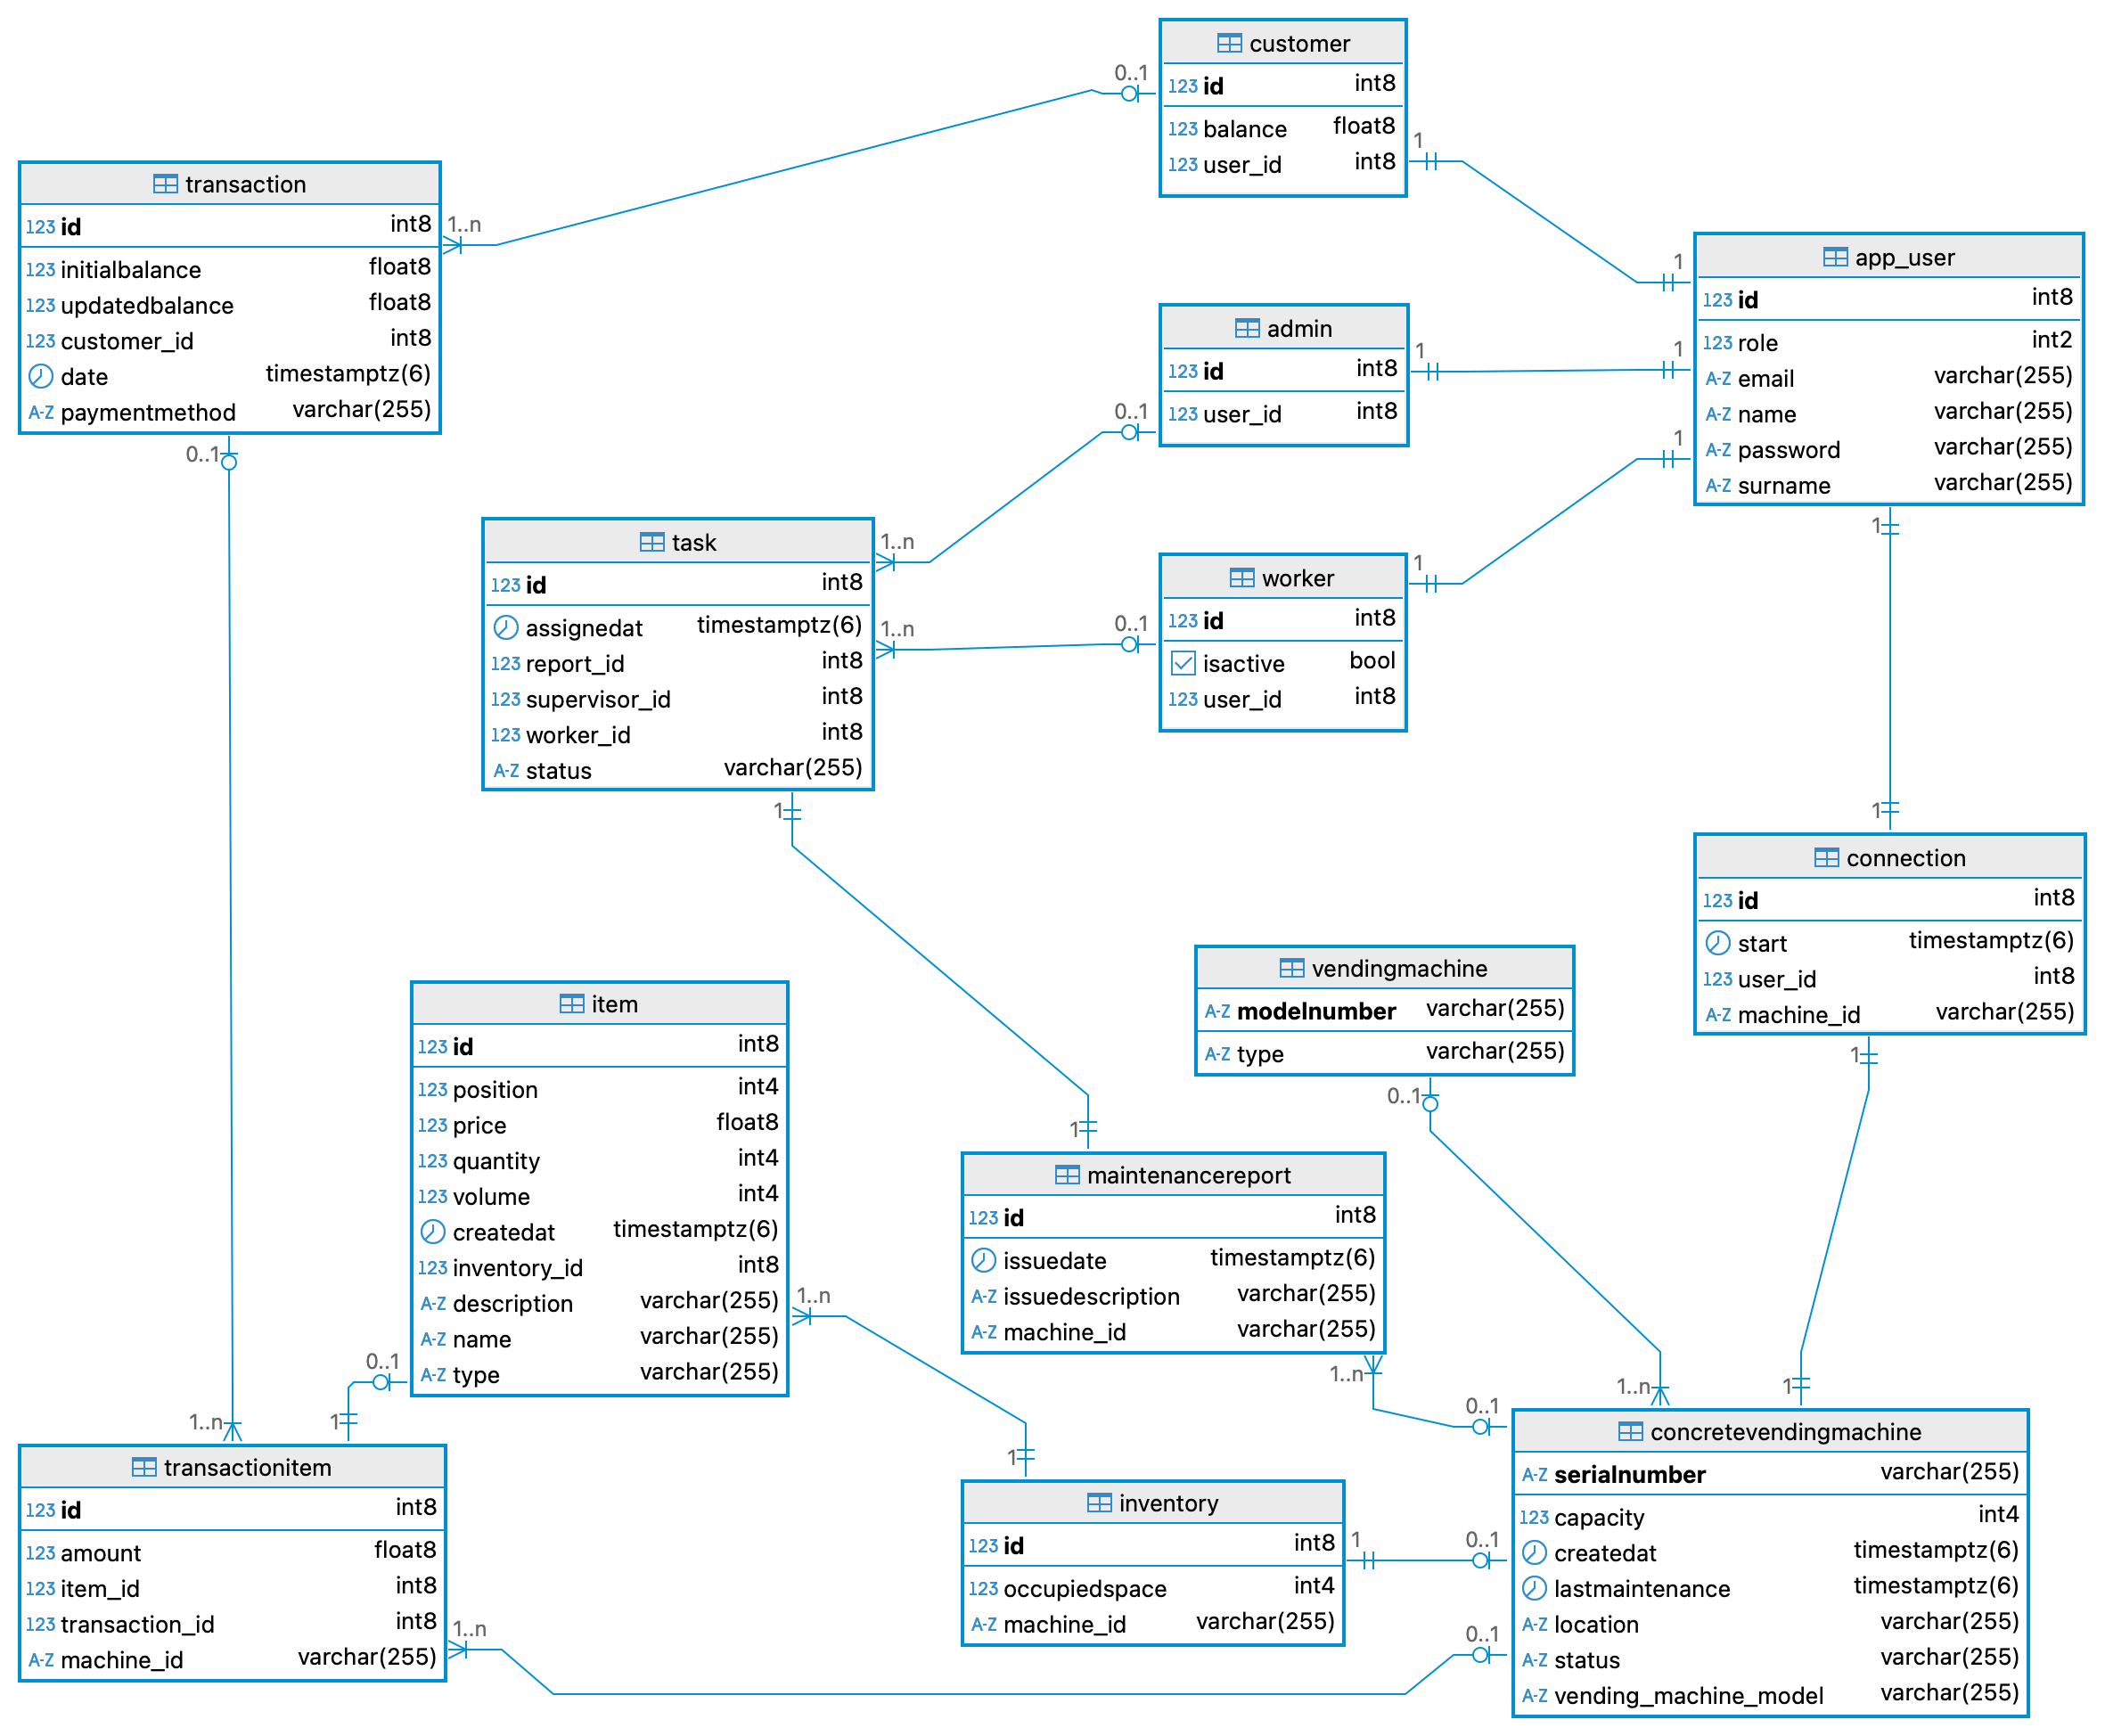
\includegraphics[width=\textwidth]{schemas/ER_Schema.png} 
    \caption{Diagramma Entità-Relazione (ER) del database di JavaBrew.}
    \label{fig:er_diagram}
\end{figure}

\subsection{Analisi Dettagliata delle Tabelle}

Lo schema è organizzato attorno a quattro aree funzionali principali: la gestione degli utenti, la gestione delle macchine, la registrazione delle transazioni e la gestione delle operazioni di manutenzione.

\subsubsection{Gestione degli Utenti}
La modellazione degli utenti adotta un approccio di \textbf{specializzazione}. Esiste una tabella base, \texttt{app\_user}, che contiene gli attributi comuni a tutti i tipi di utente.
\begin{itemize}
    \item \textbf{\texttt{app\_user}}: Funge da genitore e memorizza le informazioni anagrafiche e di accesso fondamentali, come \texttt{id}, \texttt{email}, \texttt{password}, \texttt{name}, \texttt{surname} e \texttt{role}. Il campo \texttt{role} è cruciale per distinguere le diverse tipologie di utente.
    \item \textbf{\texttt{customer}}, \textbf{\texttt{admin}}, \textbf{\texttt{worker}}: Sono tabelle di specializzazione. Ognuna ha una relazione uno-a-uno con \texttt{app\_user}, identificata dalla chiave esterna \texttt{user\_id}. Questo design permette di estendere gli attributi specifici per ogni ruolo. Ad esempio, la tabella \texttt{customer} contiene il campo \texttt{balance} per il credito, mentre la tabella \texttt{worker} ha un flag \texttt{isactive}.
\end{itemize}

\subsubsection{Gestione delle Macchine e dell'Inventario}
Anche la modellazione delle macchine da caffè segue un principio di specializzazione, separando il concetto generico di macchina da quello concreto e installato.
\begin{itemize}
    \item \textbf{\texttt{vendingmachine}}: Tabella che definisce i modelli generici di macchina, con attributi come \texttt{modelnumber} e \texttt{type}.
    \item \textbf{\texttt{concretevendingmachine}}: Rappresenta un'istanza fisica di una macchina installata in un determinato luogo. È collegata a un modello generico tramite la chiave esterna \texttt{vending\_machine\_model} e possiede attributi operativi come \texttt{serialnumber}, \texttt{location}, \texttt{status} e \texttt{capacity}.
    \item \textbf{\texttt{inventory}}: Ogni macchina concreta ha un inventario (relazione uno-a-uno). La tabella \texttt{inventory} tiene traccia dello spazio occupato (\texttt{occupiedspace}) e funge da collegamento per gli articoli.
    \item \textbf{\texttt{item}}: Contiene l'elenco dei prodotti disponibili, con attributi come \texttt{name}, \texttt{price}, \texttt{quantity} e \texttt{position}. È collegata all'inventario di una specifica macchina tramite la chiave esterna \texttt{inventory\_id}.
\end{itemize}

\subsubsection{Gestione delle Transazioni}
Questa area è responsabile della tracciabilità di tutte le operazioni finanziarie.
\begin{itemize}
    \item \textbf{\texttt{transaction}}: Memorizza l'intestazione di una transazione, come l'acquisto o una ricarica. Include l'ID del cliente (\texttt{customer\_id}), il metodo di pagamento (\texttt{paymentmethod}), e il bilancio iniziale e finale (\texttt{initialbalance}, \texttt{updatedbalance}) per una facile verifica.
    \item \textbf{\texttt{transactionitem}}: Tabella di dettaglio che realizza la relazione molti-a-molti tra transazioni e articoli. Ogni record rappresenta una riga di uno scontrino, collegando un \texttt{transaction\_id} a un \texttt{item\_id} e specificando l'importo (\texttt{amount}).
\end{itemize}

\subsubsection{Gestione Operativa}
Questo gruppo di tabelle supporta le operazioni quotidiane dell'applicazione.
\begin{itemize}
    \item \textbf{\texttt{connection}}: Traccia le connessioni attive tra un cliente e una macchina, memorizzando \texttt{user\_id}, \texttt{machine\_id} e l'orario di inizio (\texttt{start}).
    \item \textbf{\texttt{task}} e \textbf{\texttt{maintenancereport}}: Supportano il flusso di lavoro dei tecnici. Un \texttt{task} (compito) viene assegnato a un \texttt{worker} e può generare un \texttt{maintenancereport} (rapporto di manutenzione) una volta completato.
\end{itemize}

\subsection{Scelte Progettuali e Integrità dei Dati}

La progettazione del database è stata guidata da due principi chiave: la \textbf{normalizzazione} e l'\textbf{integrità referenziale}.
\begin{itemize}
    \item \textbf{Normalizzazione}: Lo schema è stato progettato per raggiungere almeno la Terza Forma Normale (3NF), riducendo al minimo la ridondanza dei dati. Ad esempio, le informazioni di un utente sono memorizzate una sola volta nella tabella \texttt{app\_user}, evitando duplicazioni.
    \item \textbf{Integrità Referenziale}: L'uso estensivo di chiavi esterne (foreign key) garantisce che le relazioni tra le tabelle siano sempre valide. Ad esempio, non è possibile creare una transazione per un cliente che non esiste, o assegnare un compito a un tecnico non presente nel sistema. Questi vincoli, imposti a livello di database, proteggono i dati da inconsistenze e sono fondamentali per la robustezza dell'intera applicazione.
\end{itemize}
